\section{Description}
% TODO
TODO: print pdfs as a function and not with bars


A binomial experiment involves $n$ independent and identical trial such that each trial can result into one of the two possible outcomes: success of failure. If $p$ is the probability of observing success in each trial, then the number of successes $X$ that can be observed out of these $n$ trials is referred to as the \textbf{binomial random variable with $n$ trials and success probability $p$}, or $B(n, p)$.

Binomial distribution is often used to estimate or determine the proportion of individuals with a particular attribute in a large population. Suppose that a random sample of $n$ units is drawn by sampling with replacement from a finite population or by sampling without replacement from a large population. The number of units that contain the attribute of interest in the sample follows a normal distribution.

If the sample was drawn without replacement from a small finite population, the hypergeometric distribution should be used instead of the binomial.

\subsection{Probability mass function}
The probability of observing $k$ successes out of $n$ trials is given by the following probability mass function
\[
	P(X = k \mid n, p) = \binom{n}{k}p^{k}(1 - p)^{n - k}, \quad k = 0, 1, \ldots, n
\]

Binomial's pmf is right-skewed when $p < 0.5$, left-skewed when $p > 0.5$ and symmetric when $p = 0.5$.

% For the future: on image and floats positioning
% https://tex.stackexchange.com/questions/278727/split-subfigures-over-multiple-pages/278748
% https://tex.stackexchange.com/questions/16207/image-from-includegraphics-showing-up-in-wrong-location/16211
\begin{figure}[H]
	\centering
	\begin{subfigure}[b]{0.45\textwidth}
		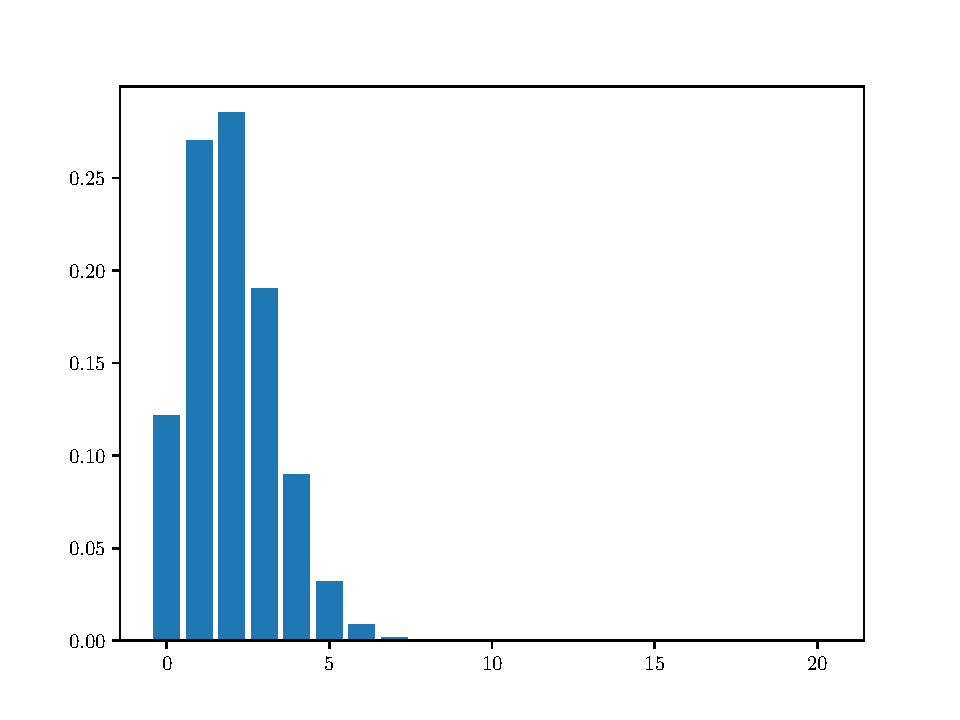
\includegraphics[width=\textwidth]{discrete/binomial/pmf_20_01.pdf}
		\caption{$B(20, 0.1)$}
	\end{subfigure}
	\begin{subfigure}[b]{0.45\textwidth}
		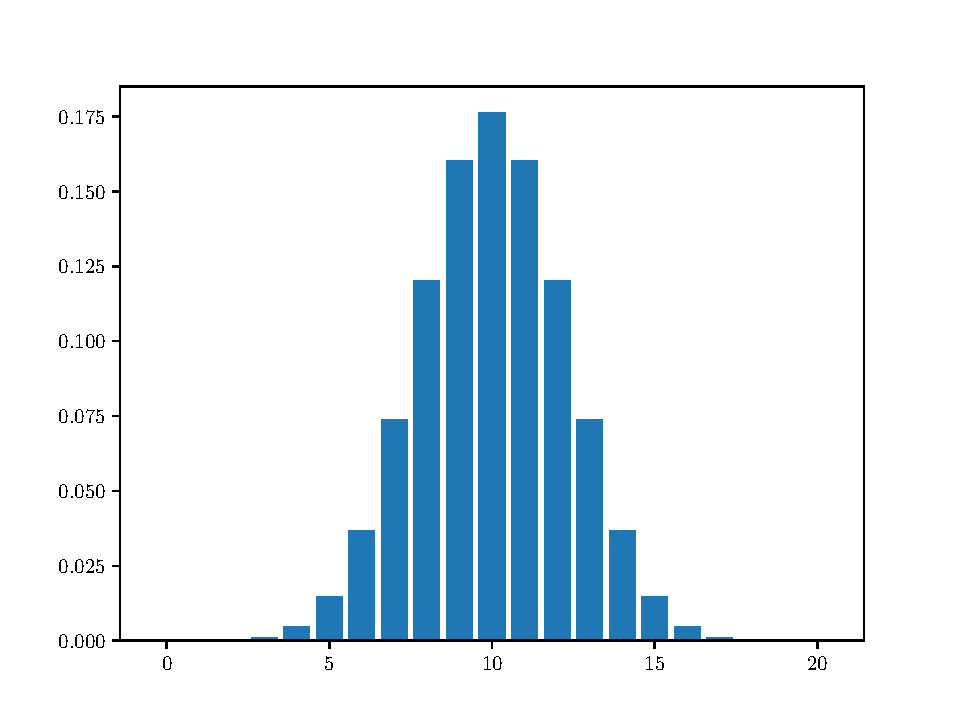
\includegraphics[width=\textwidth]{discrete/binomial/pmf_20_05.pdf}
		\caption{$B(20, 0.5)$}
	\end{subfigure}
	\begin{subfigure}[b]{0.45\textwidth}
		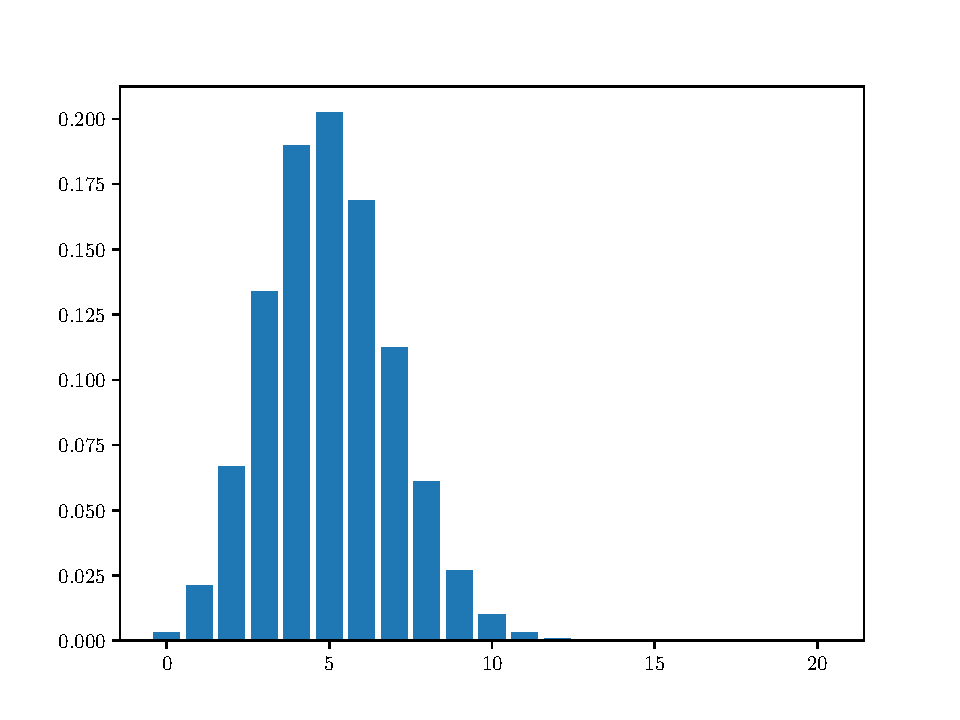
\includegraphics[width=\textwidth]{discrete/binomial/pmf_20_025.pdf}
		\caption{$B(20, 0.25)$}
	\end{subfigure}
	\begin{subfigure}[b]{0.45\textwidth}
		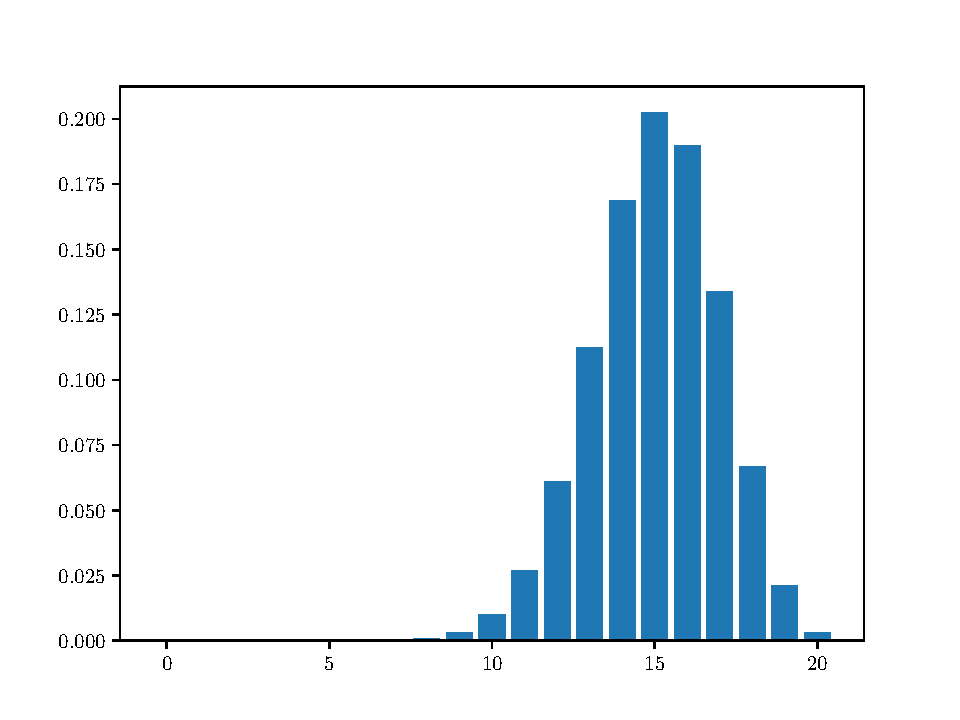
\includegraphics[width=\textwidth]{discrete/binomial/pmf_20_075.pdf}
		\caption{$B(20, 0.75)$}
	\end{subfigure}
	\begin{subfigure}[b]{0.45\textwidth}
		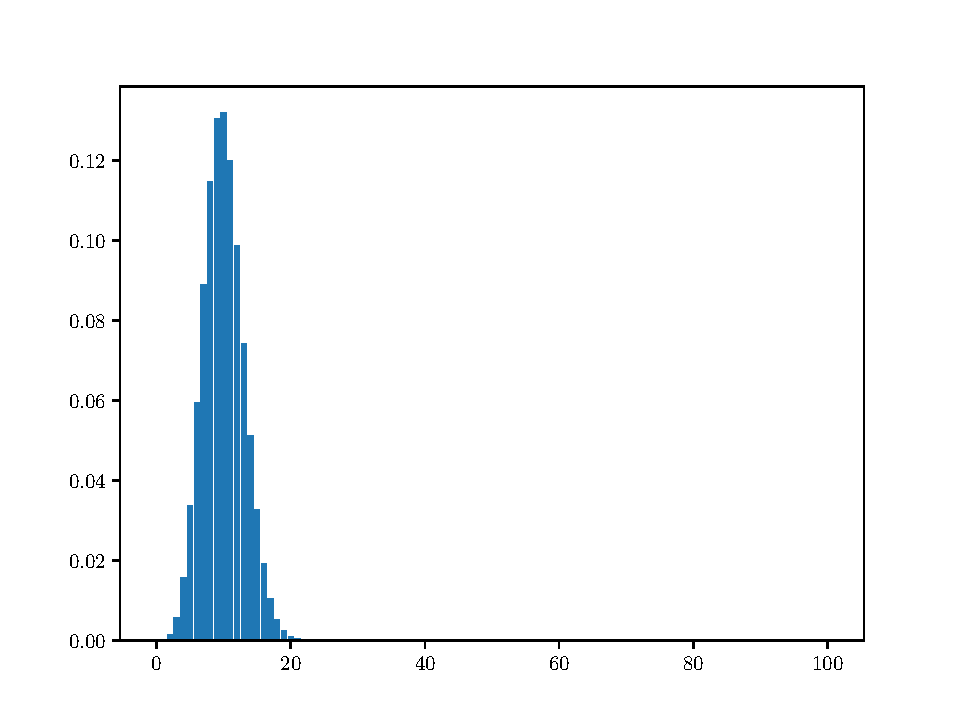
\includegraphics[width=\textwidth]{discrete/binomial/pmf_100_01.pdf}
		\caption{$B(100, 0.1)$}
	\end{subfigure}
	\begin{subfigure}[b]{0.45\textwidth}
		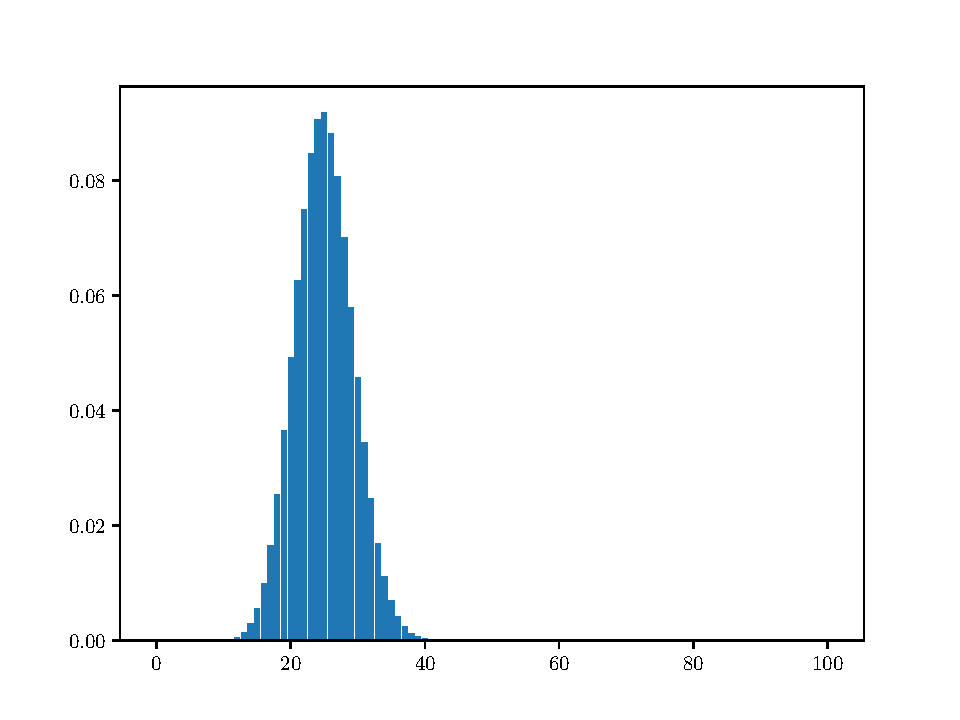
\includegraphics[width=\textwidth]{discrete/binomial/pmf_100_025.pdf}
		\caption{$B(100, 0.25)$}
	\end{subfigure}
	\caption{Binomial distribution}
\end{figure}

\begin{figure}[H]
	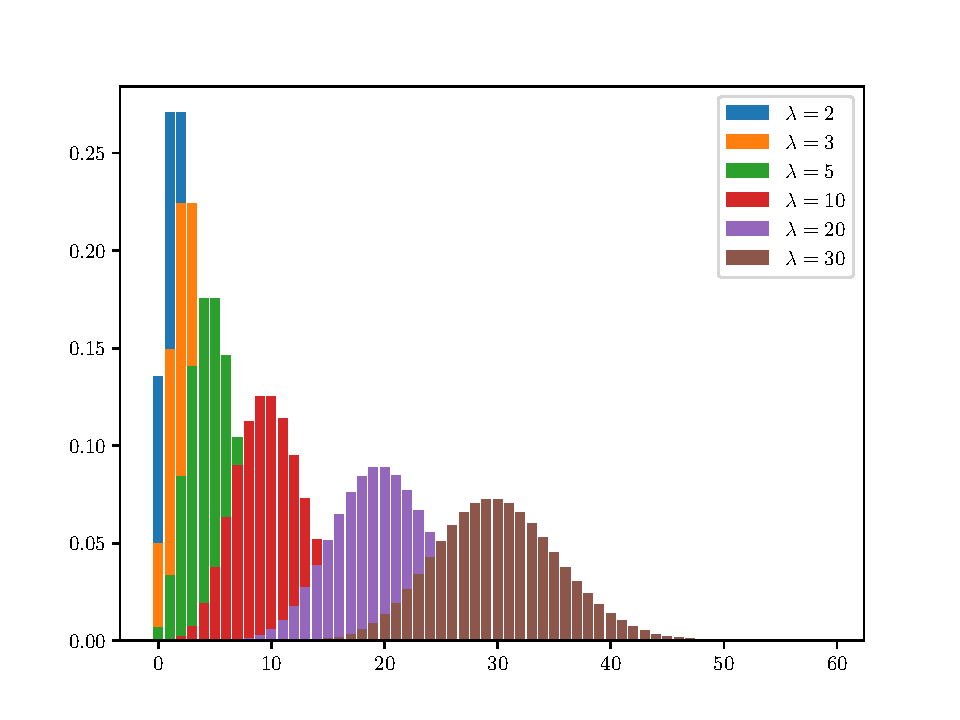
\includegraphics[width=\textwidth]{discrete/binomial/pmf_all.pdf}
	\caption{$P(X = k \mid n, p) = \binom{n}{k}p^{k}(1 - p)^{n - k}, \quad k = 0, 1, \ldots, n$}
\end{figure}

\subsection{Cumulative distribution function}
\[
	P(X \leq k \mid n, p) = \sum_{i = 0}^{k} \binom{n}{i}p^{i}(1 - p)^{n - i}, \quad k = 0, 1, \ldots, n
\]

\begin{figure}[H]
	\centering
	\begin{subfigure}[b]{0.45\textwidth}
		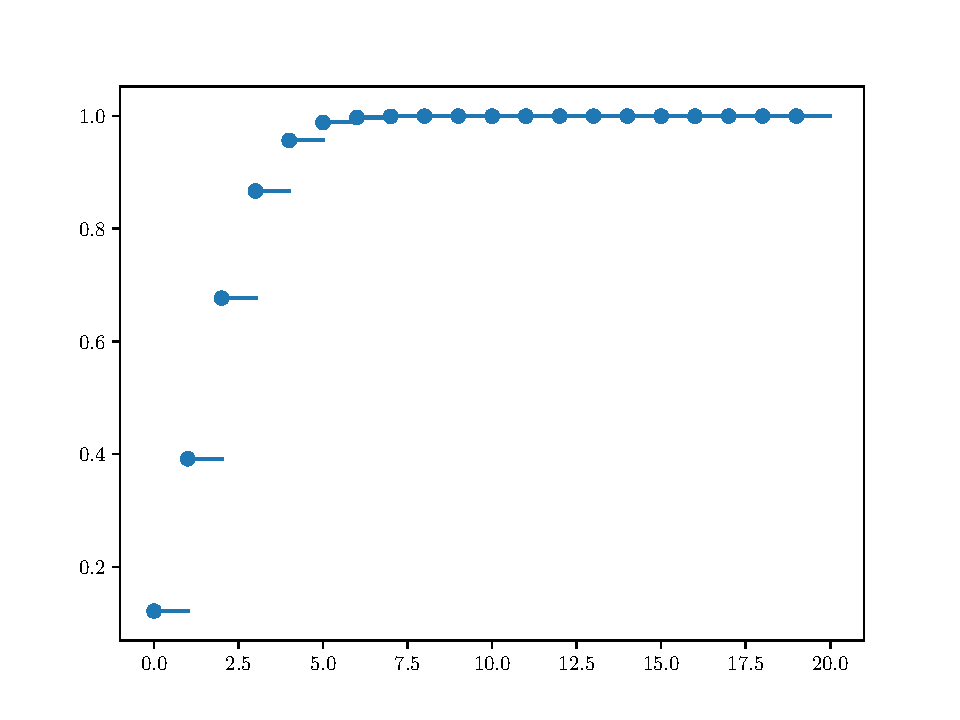
\includegraphics[width=\textwidth]{discrete/binomial/cdf_20_01.pdf}
		\caption{$B(20, 0.1)$}
	\end{subfigure}
	\begin{subfigure}[b]{0.45\textwidth}
		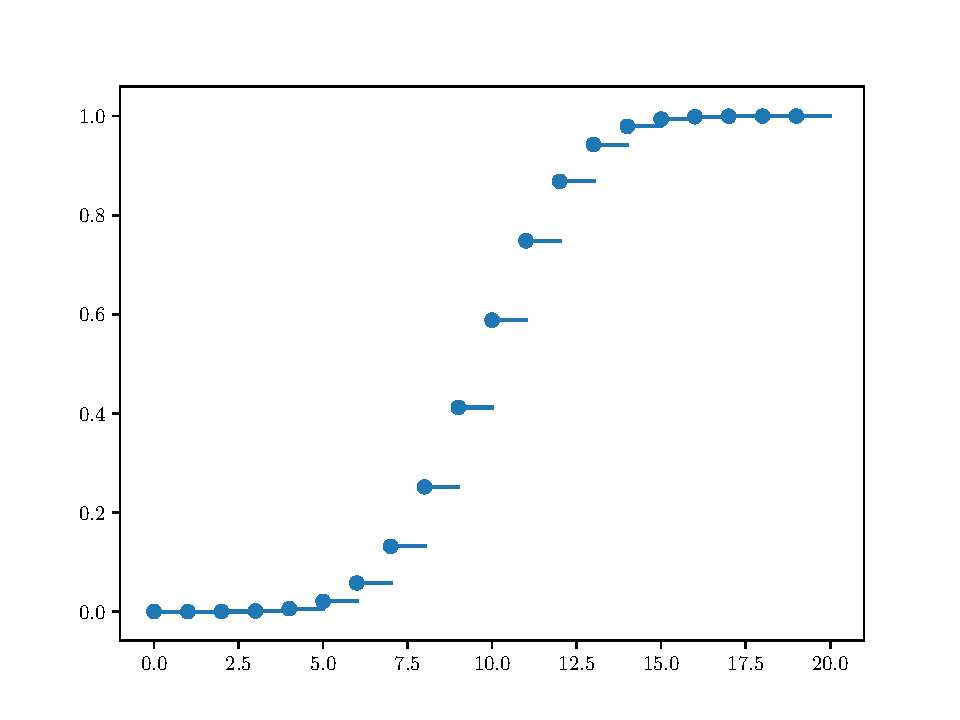
\includegraphics[width=\textwidth]{discrete/binomial/cdf_20_05.pdf}
		\caption{$B(20, 0.5)$}
	\end{subfigure}
	\begin{subfigure}[b]{0.45\textwidth}
		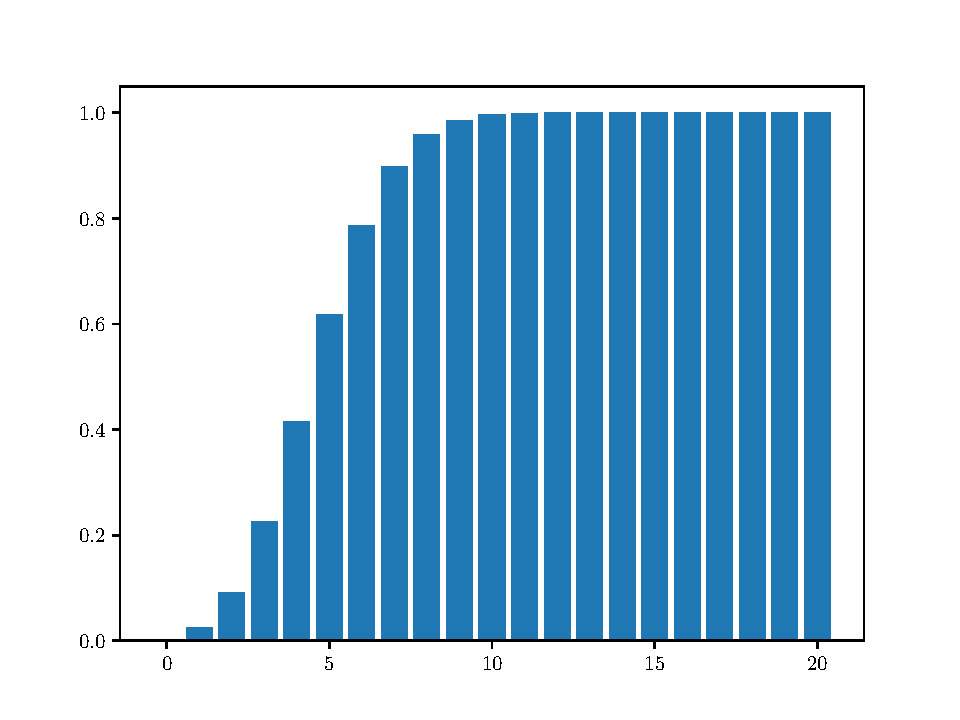
\includegraphics[width=\textwidth]{discrete/binomial/cdf_20_025.pdf}
		\caption{$B(20, 0.25)$}
	\end{subfigure}
	\begin{subfigure}[b]{0.45\textwidth}
		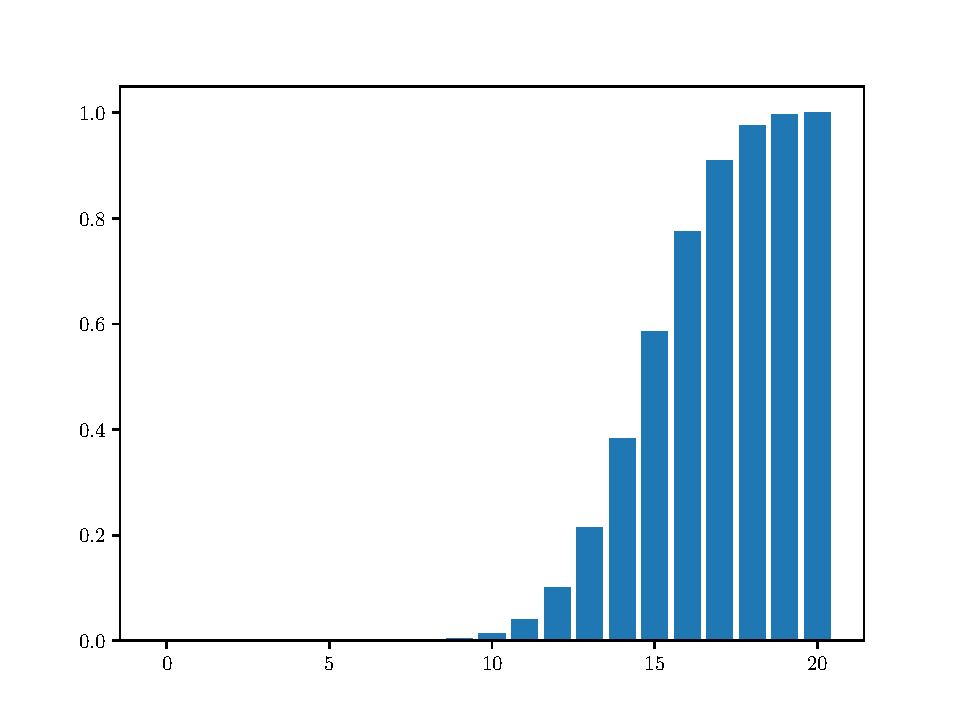
\includegraphics[width=\textwidth]{discrete/binomial/cdf_20_075.pdf}
		\caption{$B(20, 0.75)$}
	\end{subfigure}
	\begin{subfigure}[b]{0.45\textwidth}
		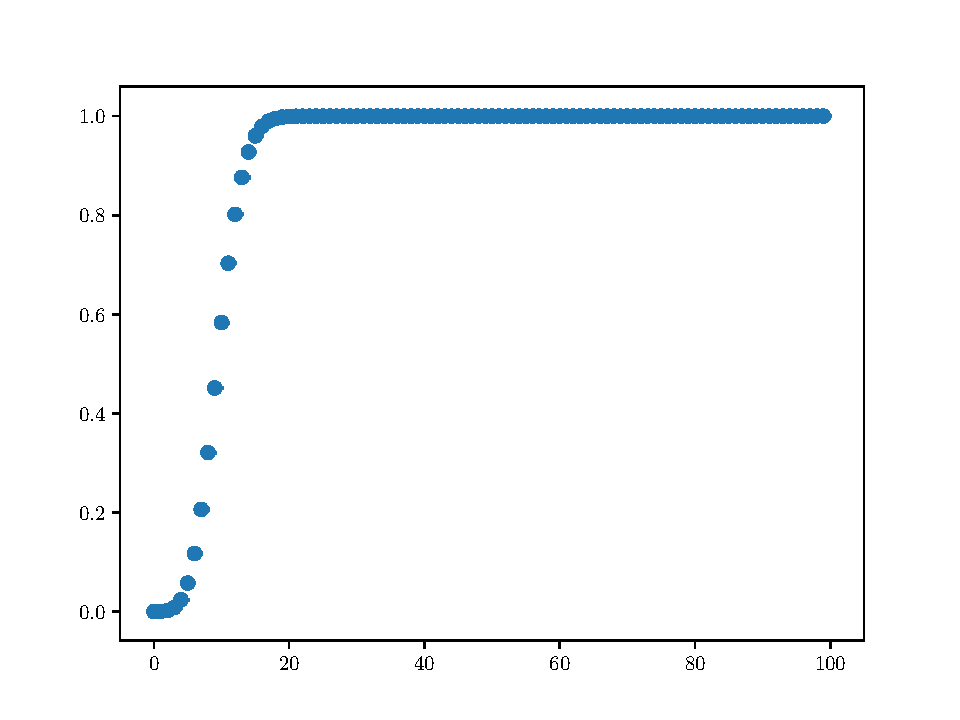
\includegraphics[width=\textwidth]{discrete/binomial/cdf_100_01.pdf}
		\caption{$B(100, 0.1)$}
	\end{subfigure}
	\begin{subfigure}[b]{0.45\textwidth}
		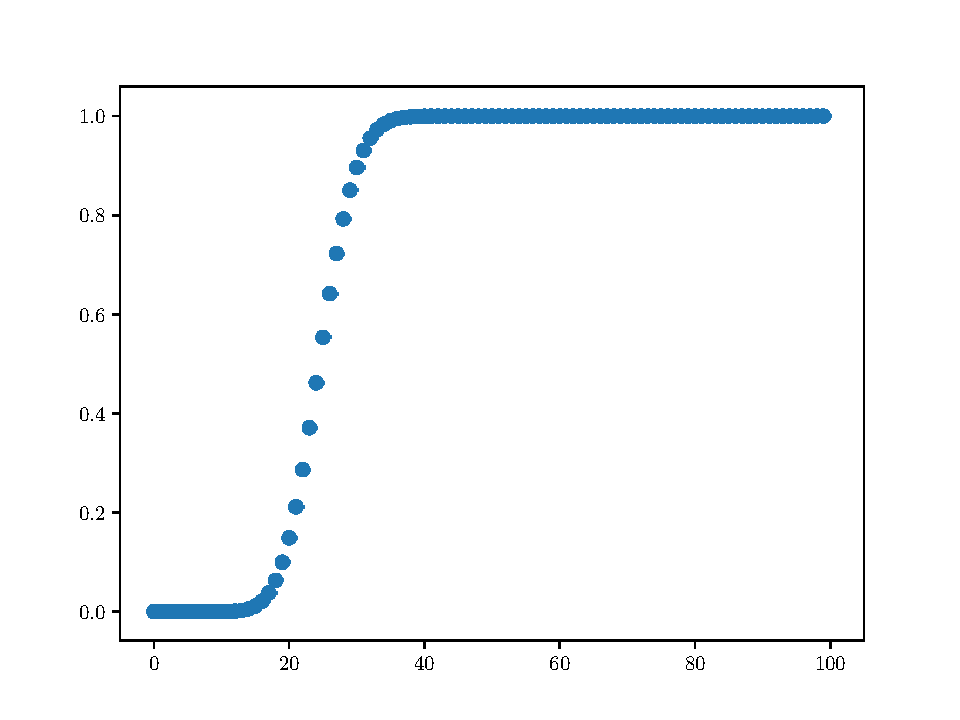
\includegraphics[width=\textwidth]{discrete/binomial/cdf_100_025.pdf}
		\caption{$B(100, 0.25)$}
	\end{subfigure}
	\caption{Binomial distribution}
\end{figure}

\begin{figure}[H]
	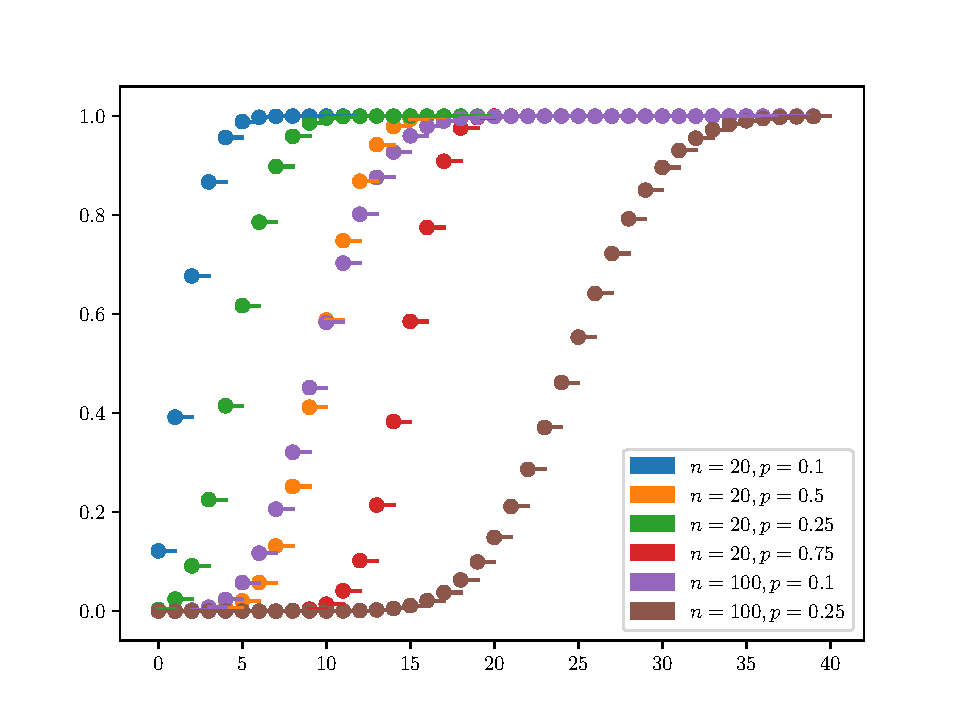
\includegraphics[width=\textwidth]{discrete/binomial/cdf_all.pdf}
	\caption{$P(X \leq k \mid n, p) = \sum_{i = 0}^{k} \binom{n}{i}p^{i}(1 - p)^{n - i}, \quad k = 0, 1, \ldots, n$}
\end{figure}

\section{Moments}

\begin{tabularx}{\textwidth}{s X}
	\hline
	Mean & $np$ \\\hline
	Variance & $np(1 - p)$\\\hline
\end{tabularx}

\section{Properties}
\begin{enumerate}
	\item Let $X_1, \ldots, X_m$ be independent random variables with $X_i \sim B(n_i, p), \ i = 1, 2, \ldots, m$. Then,
	\[
	\sum_{i = 1}^m X_i \sim B\left(\sum_{i = 1}^m n_i, p\right)
	\]
	\item Let $X_1, \ldots, X_m$ be independent Bernoulli$(p)$ random variables with success probability $p$. That is: $P(X_i = 1) = p, \ P(X_i = 0) = 1 - p, \ i = 1, \ldots, n$. Then,
	\[
	\sum_{i = 1}^m X_i \sim B\left(n, p\right)
	\]
\end{enumerate}

\section{Examples}
\begin{example}
	A fair die is rolled $n$ times.
	\begin{itemize}
		\item The probability of obtaining exactly one 6 is $n\left(\frac{1}{6}\right)\left(\frac{5}{6}\right)^{n - 1}$.
		\item The probability of obtaining no 6 is $\left(\frac{5}{6}\right)^n$.
		\item The probability of obtaining at least one 6 is $1 - \left(\frac{5}{6}\right)^n$.
		\item The number of trials needed for the probability of at least one 6 to be $\geq \frac{1}{2}$ is given by the smallest integer $n$ such that $1 - \left(\frac{5}{6}\right)^n \geq \frac{1}{2}$, so that $n \geq \frac{\log 2}{\log 1.2} \approx 3.8$.
	\end{itemize}
\end{example}

